\Chapter{A frontend megvalósítása}

A fejezet a felhasználóhoz közeli grafikus elemek elkészítését, azok működését mutatja be.

\Section{Felhasznált technológiák}

A felület létrehozásához \textit{TypeScript} \cite{typescript} programozási nyelvet használtam és \textit{React} \cite{react} könyvtárat.

\SubSection{TypeScript}

A \textit{TypeScript} egy nyílt forráskódú nyelv, amely a JavaScript-re, a világ egyik leggyakrabban használt nyelvére épít rá, statikus típusdefiníciók hozzáadásával bővíti azt. Tehát minden jól működő JavaScript kód egyben jó TypeScript kód is. Viszont lehet kapunk pár típussokkal kapcsolatos hibát de pont emiatt szerettem volna használni, hogy átláthatóbb kódot írjak és kevesebb időt kelljen töltenem hibakereséssel. \bigskip

A típusok biztosítják nekünk az objektum alakjának leírását, jobb dokumentációt nyújtanak, és elősegíti a TypeScript számára, hogy ellenőrizze, a kód megfelelően működik.\bigskip

Az típusok definiálása opcionális TypeScript-ben, de azért jó ha írunk típusokat mert lehetővé teszi, hogy sok energiát spóroljunk azzal, hogy maga a kód rövidebb, kifejezőbb tud lenni.

\SubSection{React}

Az eredetileg a Facebook számára kifejlesztett React egy JavaScript könyvtár, amely single-page (SPA, \textit{Single Page Application}) alkalmazások készítésére szokás használni, azáltal, hogy a UI-t komponensekre osztja fel. Mivel csak a HTML és a JavaScript minimális megértését igényli, a React mint front-end webfejlesztő eszköz egyre népszerűbb, ma már talán a legelterjedtebb JavaScript könyvtár. \bigskip

Pont emiatt esett rá a választásom, mert rendkívül felkapott és rengeteg ember használja, így sok helyen lehet hozzá forrást találni, valamint nagyon gyors.

\Section{Az alkalmazás komponensei}

Az oldalon 5 fő komponens található, amelyek megvalósítják a funkciókat. A többi komponens ezekben kerül hivatkozásra, tehát ezeknek a gyerekei. A következő szakaszok ezen komponenseket taglalják.

\SubSection{Authentication}

Ebben a komponenseben történik a bejelentkezés és regisztráció is egyszerre. Egy új felhasználónak ide kell jönnie először mivel csak bejelentkezve érhetőek el a funkciók.

\begin{figure}[h!]
    \centering
    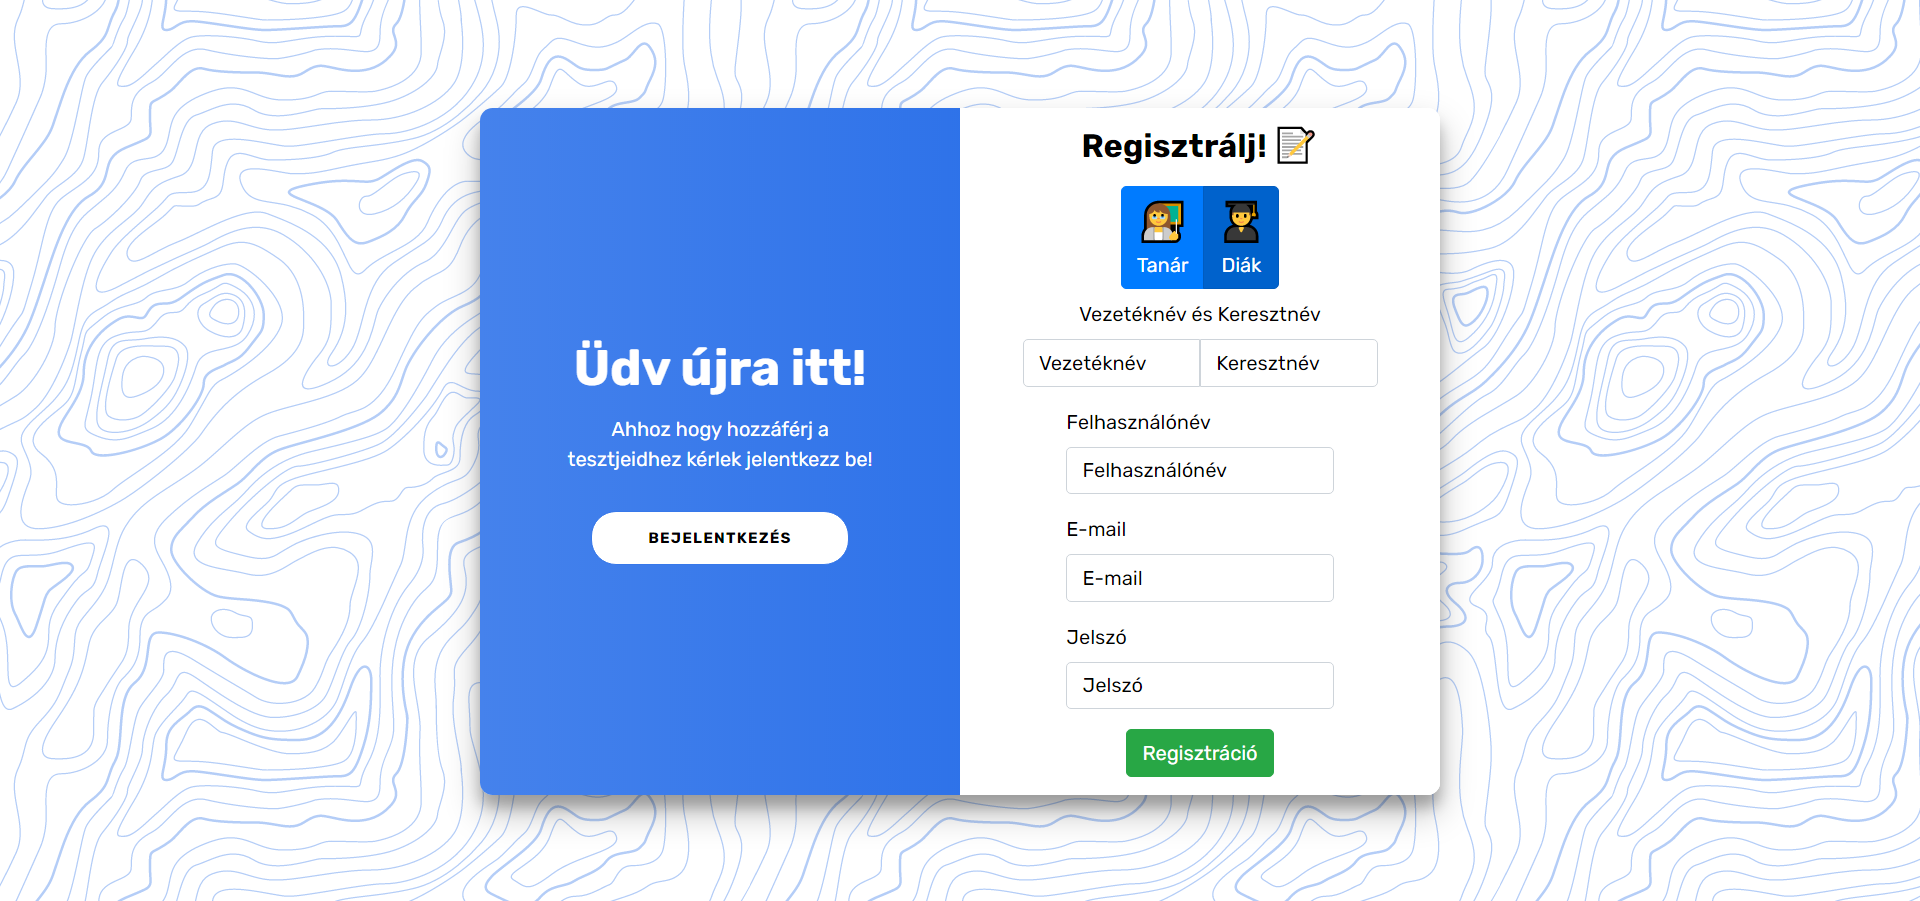
\includegraphics[width=\linewidth]{images/signin.png}
    \caption{Regisztráció}
    \label{fig:signin}
\end{figure}

Legelőször is regisztrálni kell (\prettyref{fig:signin}. ábra). Ehhez szükséges megadni, hogy diák vagy tanárként regisztrálunk, a teljes nevünket, egy tetszőleges felhasználónevet egy email címet és a jelszót. Majd ezt követően kapunk egy email-t amiben van egy hivatkozás, aminek a segítségével vissza tudjuk igazolni a regisztrációt. Erre azért van szükség, mert így biztos mi regisztráljuk az email címünkkel és nem más.

\begin{figure}[h!]
    \centering
    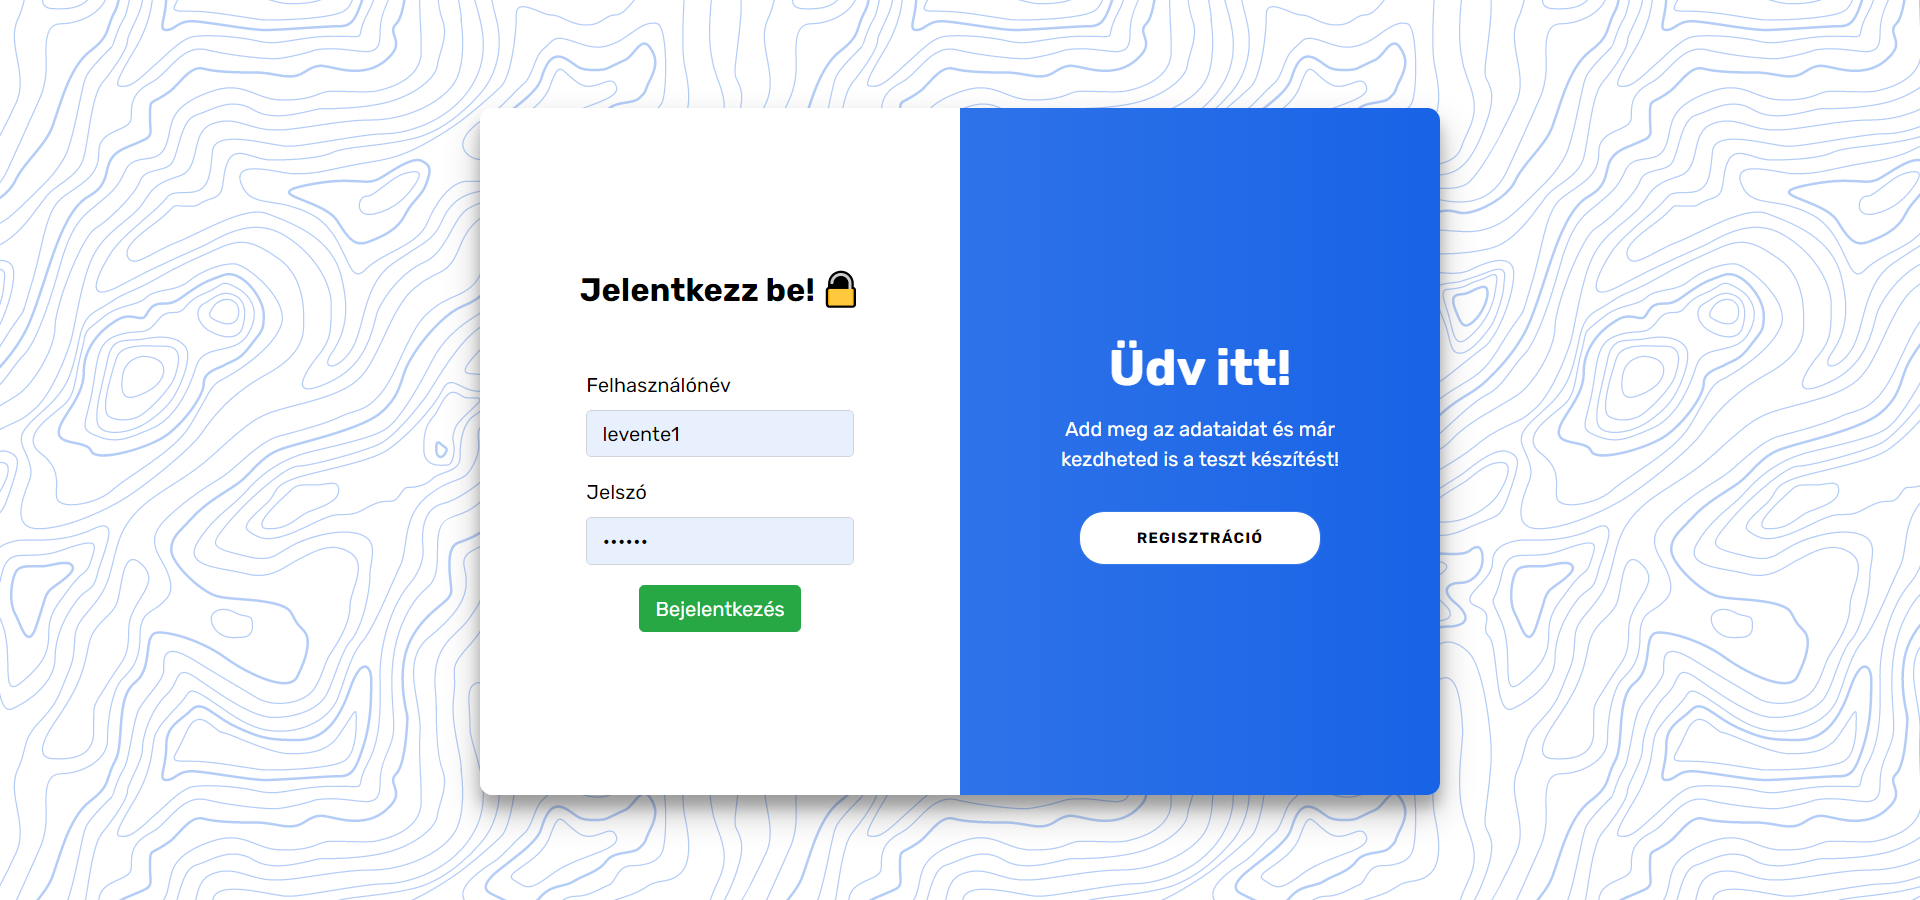
\includegraphics[width=\linewidth]{images/login.png}
    \caption{Bejelentkezés}
    \label{fig:login}
\end{figure}

Ez után, ha sikeresen megerősítettük az email címünket, bejelentkezhetünk a felhasználónevünkkel és jelszavunkkal (\prettyref{fig:login}. ábra).
A bejelentkezés és regisztrációs űrlapon is van validáció. Ha a mezők üresek, akkor nem küldi el az adatokat, emellett ha helytelen az email cím nem enged regisztrálni vele. Valamint hibaüzenetet ír ki, ha úgy próbálunk bejelentkezni, hogy nincs visszaigazolva az email címünk vagy rossz felhasználónevet, jelszót próbáltunk beírni.

\SubSection{Home}

Bejelentkezés után automatikusan átkerülünk a főoldalra (\prettyref{fig:home}. ábra) ahol láthatjuk a teljes nevünket, hanyas szintűek vagyunk a pontjaink alapján és, hogy hány darab kitöltött és kitöltetlen tesztünk van.

\begin{figure}[h!]
	\centering
	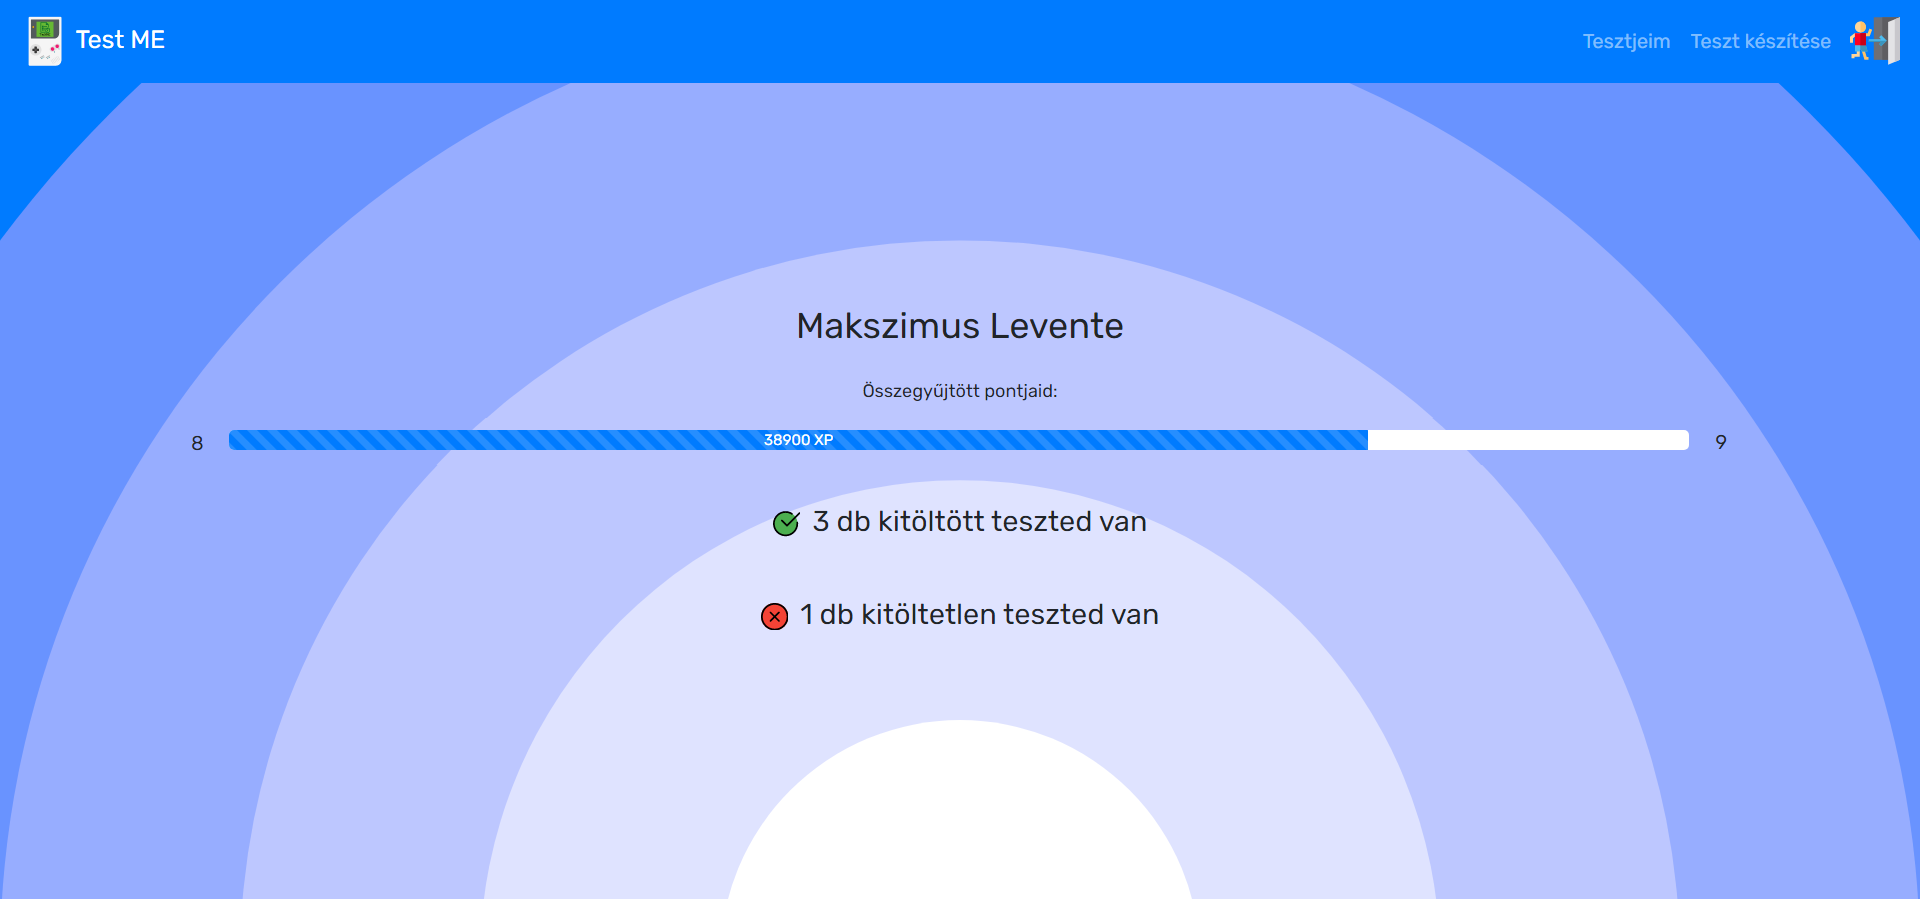
\includegraphics[width=\linewidth]{images/home.png}
	\caption{Főoldal}
	\label{fig:home}
\end{figure}

\noindent Itt láthatjuk egyben a fontos adatokat. A szint meghatározása úgy történik hogy 5000 pontonként lehet egy szintet lépni, tehát például az itt szereplő képen 8 és 9-es szint között vagyunk. Ez azt jelenti, hogy 35000-től több de 40000-től kevesebb pontom van.

\SubSection{CreateTest}

Ebben a komponenseben történik a tesztek létrehozása.

\begin{figure}[H]
    \centering
    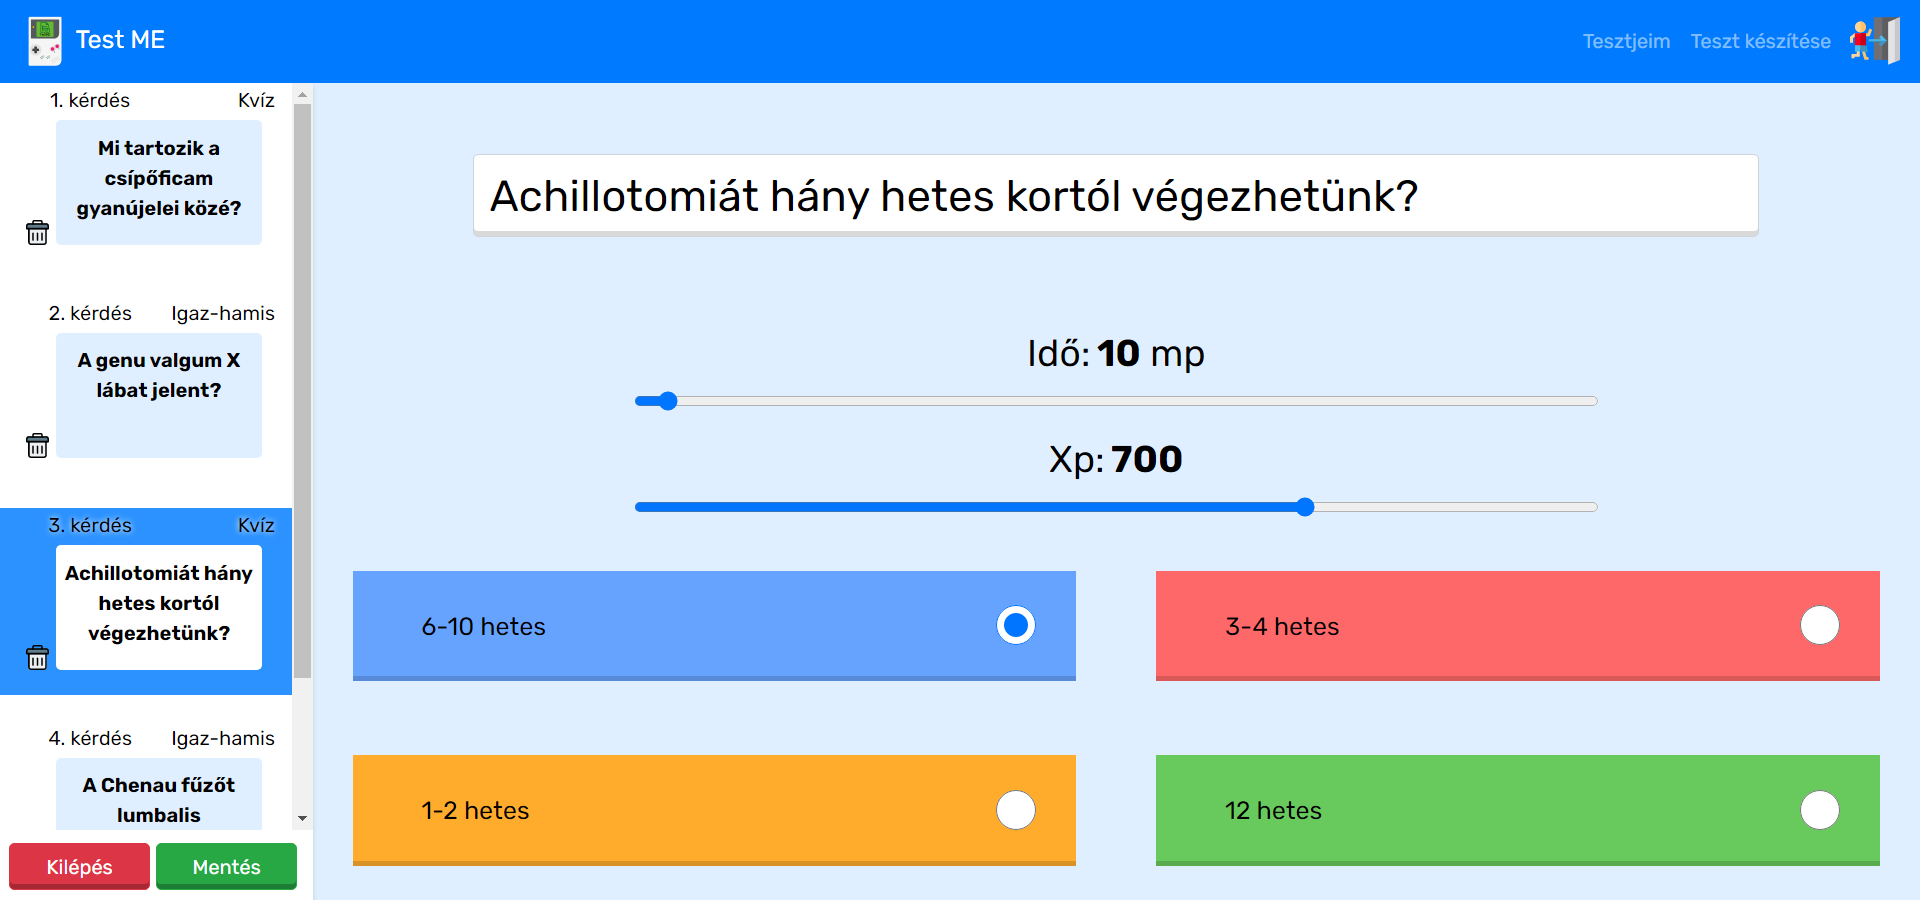
\includegraphics[width=\linewidth]{images/make_test1.png}
    \caption{Teszt készítés}
    \label{fig:make_test1}
\end{figure}

\noindent Két részre van osztva a felület (\prettyref{fig:make_test1}. ábra). A bal oldali sávban vannak az eddig hozzáadott kérdéseink amiket létre tudunk hozni, törölni, kiválasztani majd szerkeszteni. A téglalapokban látszódik a feltett kérdésünk, fölötte pedig, hogy hanyadik és milyen típusú. A jobb oldali részen pedig, ha rákattintunk egy létrehozott kérdésre ide tölti be a kérdés adatait. Így tudjuk kitölteni vagy módosítani. Itt adjuk meg mi legyen a kérdés, mik a lehetséges válaszok, ezek közül melyik a jó, mennyi időt engedünk, hogy válaszoljanak rá és mennyi pontot adunk érte. Ez a pont viszont teszt kitöltésnél idő és válasz alapján dől el, hogy mennyit kap belőle a kitöltő. Tehát például ezt a 700 pontot akkor kapja meg, ha azonnali jó választ ad. Minél többet gondolkodik a kérdésen, annál kevesebbet kap meg belőle. Tehát itt, egy maximum értéket kell meghatározni.

\begin{figure}[H]
    \centering
    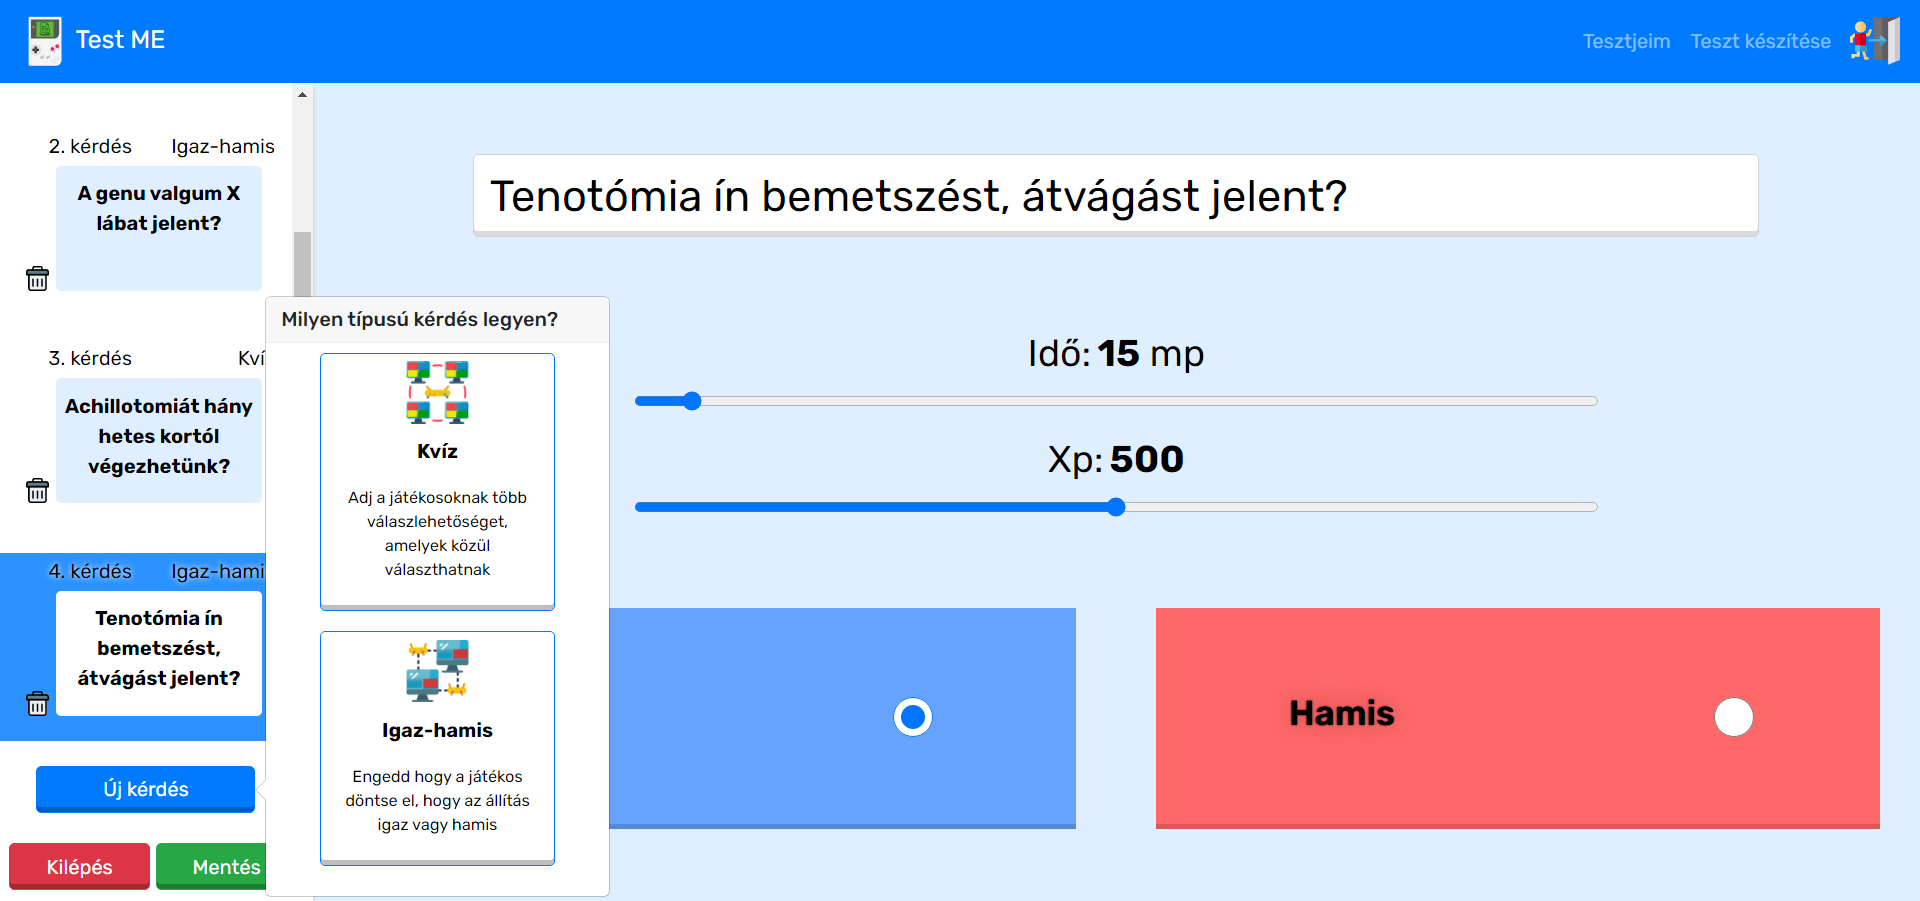
\includegraphics[width=\linewidth]{images/make_test2.png}
    \caption{Kérdés típus választás}
    \label{fig:make_test2}
\end{figure}

Kétféle kérdés típus közül lehet választani (\prettyref{fig:make_test2}. ábra). Van a kvíz kérdés, aminél egy kérdésre négy válaszlehetőség van és egy jó válasz. Valamint van az igaz-hamis aminél értelem szerűen meg kell adni, hogy a feltett kérdés igaz vagy hamis.

\begin{figure}[H]
    \centering
    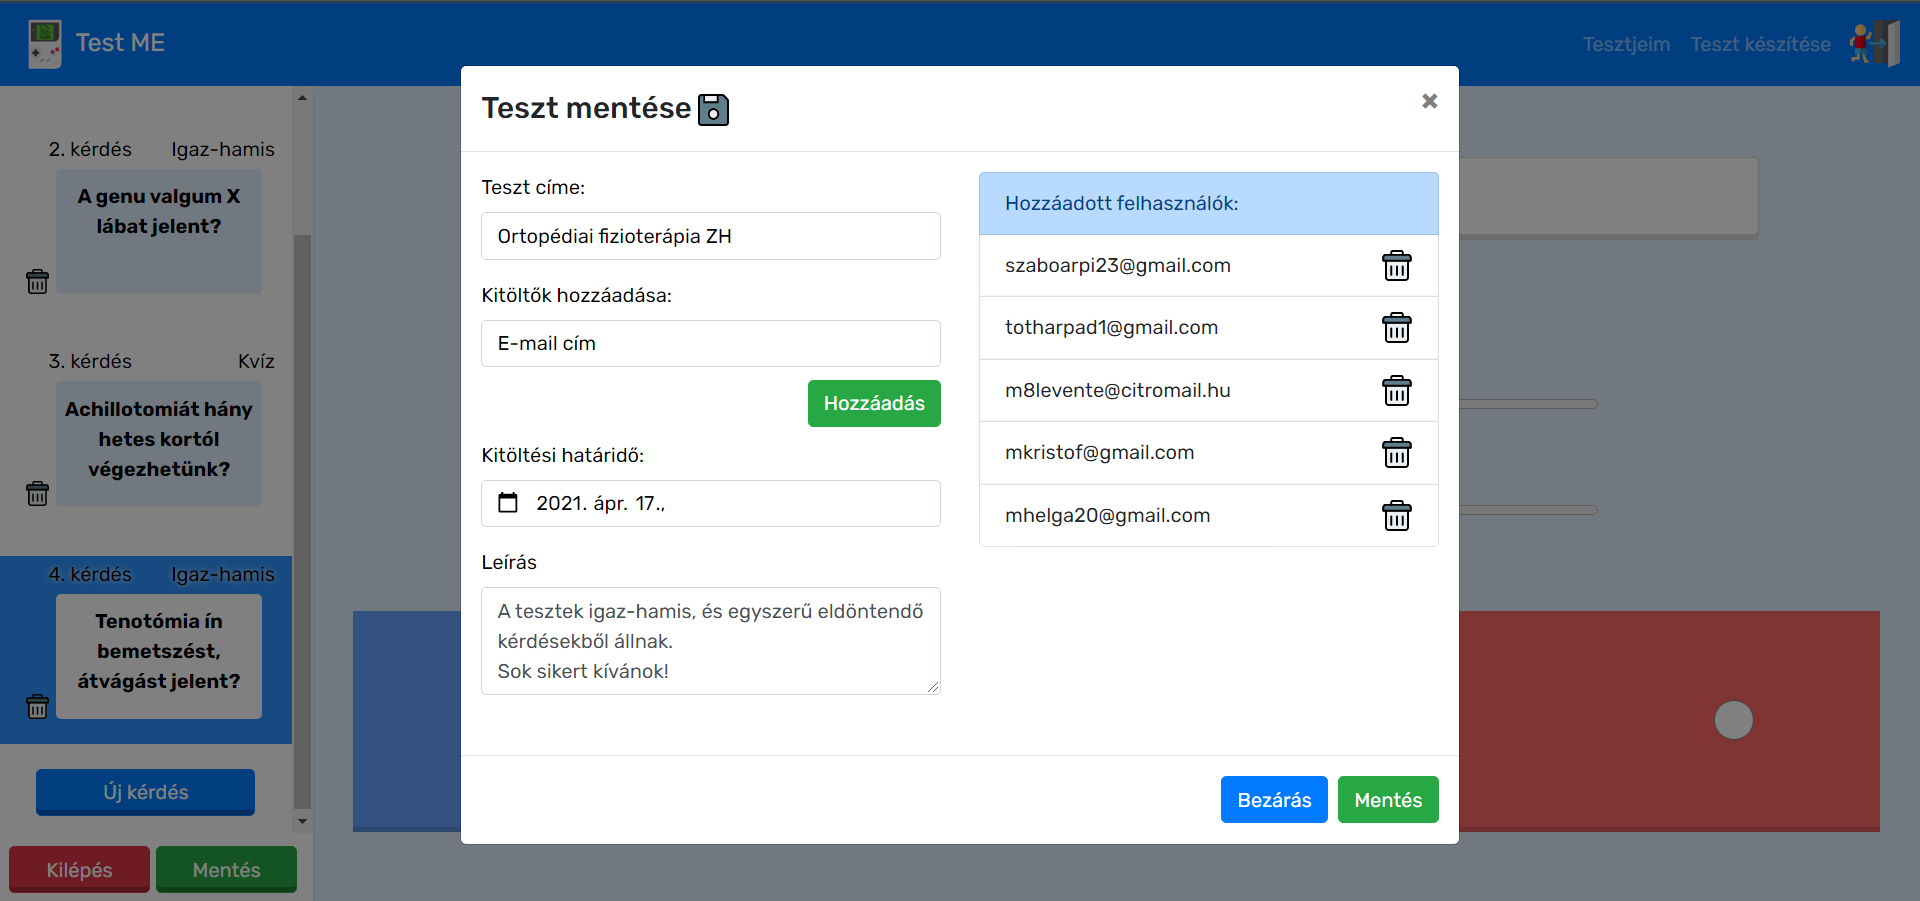
\includegraphics[width=\linewidth]{images/make_test3.png}
    \caption{Teszt mentése}
    \label{fig:make_test3}
\end{figure}

Ezután, ha mindennel megvagyunk és rákattintunk a mentés gombra, majd felugrik egy űrlap (\prettyref{fig:make_test3}. ábra) ahova be kell írni az alap teszthez tartozó adatokat. Ezek közé tartozik a teszt címe, kitöltési határideje, leírása és a felhasználók email címe, akiknek ki kell töltenie a tesztet. Az utóbbit úgy tudjuk megtenni, hogy beírjuk a mezőbe és a hozzáadás gombbal tudjuk hozzáadni az oldalsó listához. Emellett törölni is tudjuk őket, ha véletlenül helytelenül írtunk volna be egy email-t.

\subsubsection{MyTests}

Ezt követően ha elmentettük a tesztet átkerülünk a ,,Tesztjeim'' nevű oldalra (\prettyref{fig:my_tests}. ábra), ahol megnézhetjük a tesztjeinket amiket ki kell töltenünk vagy amiket mi kreáltunk.

\begin{figure}[H]
	\centering
	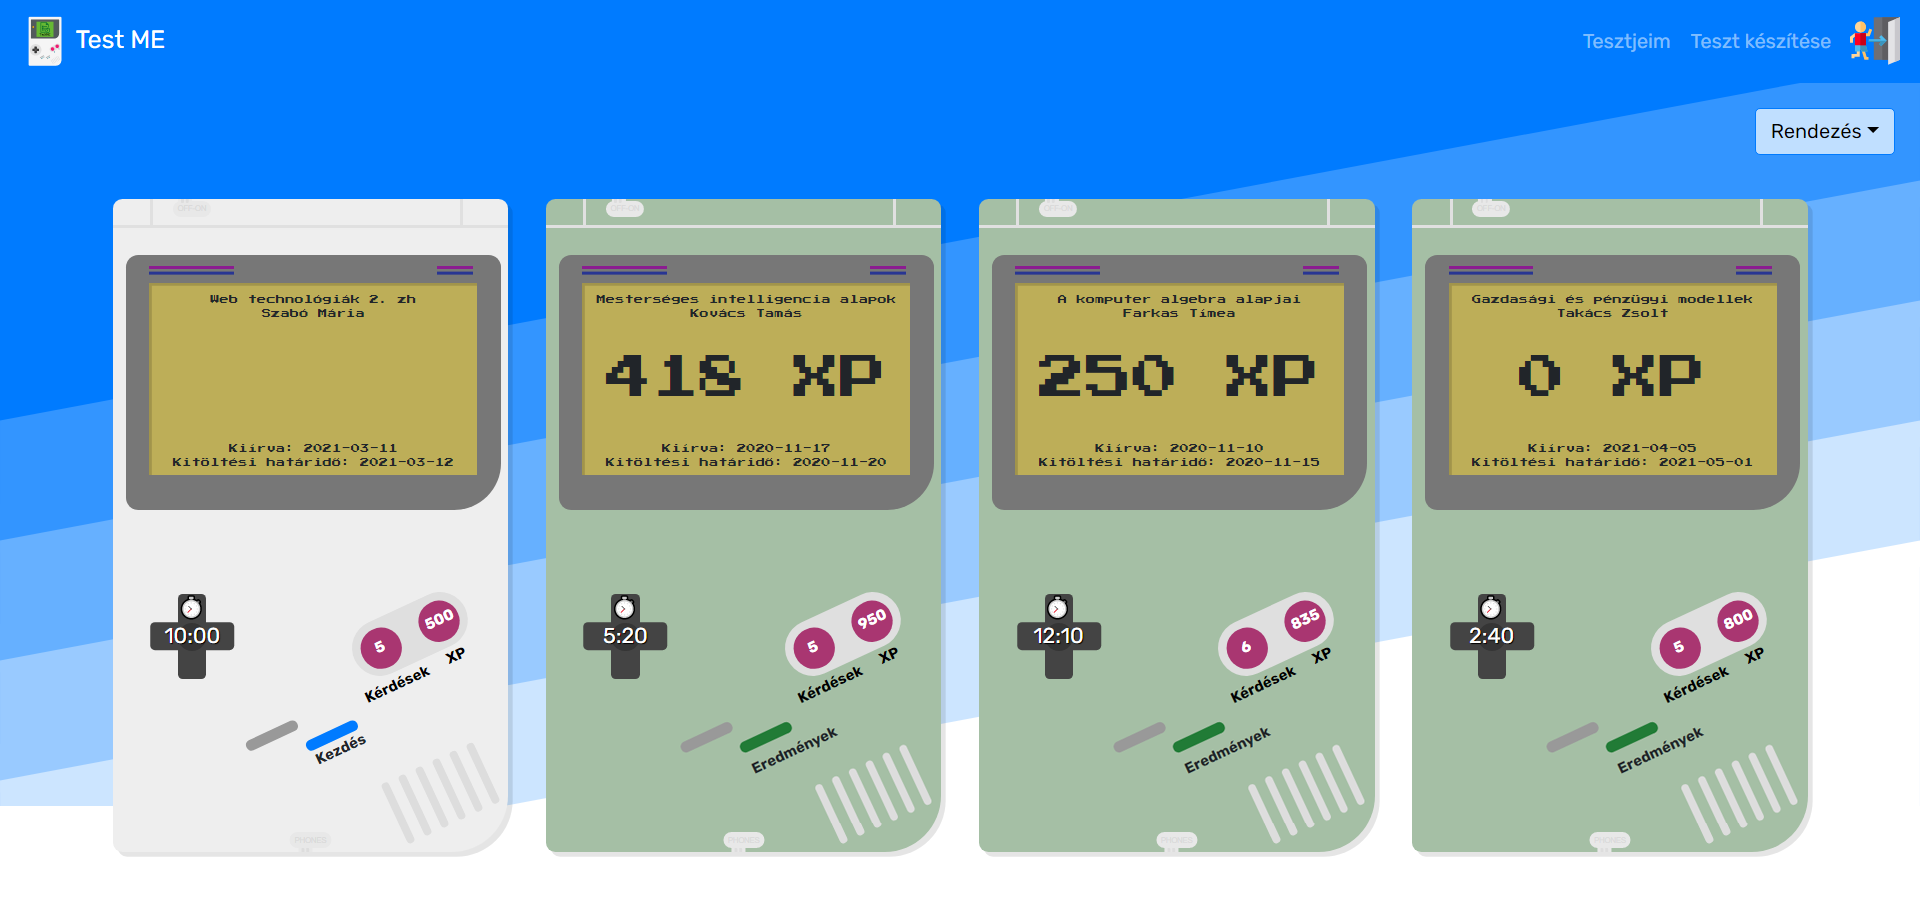
\includegraphics[width=\linewidth]{images/my_tests.png}
	\caption{Saját tesztek}
	\label{fig:my_tests}
\end{figure}

\noindent Itt a játékosság szemléltetése végett minden tesztet egy Game Boy ábrázol. Itt látszódik rajta a teszt címe, hogy ki készítette és mikor, mi a kitöltési határidő, mennyi idő van az összes kérdésre egybevéve, hány kérdés van és, hogy mennyi pont jár az az összes kérdésre ha hibátlanul és gyorsan válaszolunk. \newline

Azt, hogy melyik kérdést hoztuk mi létre és melyik az amelyiket nekünk kell kitölteni, azt két helyen is észre lehet venni. Először is látjuk, hogy a teszt címe alatt a saját nevük van, második pedig hogy a ,,Kezdés'' gomb helyett rögtön azt látjuk hogy ,,Eredmények''. Viszont ugyan ez az ,,Eredmények'' gomb lesz ott akkor is, ha egy tesztet már kitöltöttünk és később vissza szeretnénk nézni, hogy mások hogy teljesítettek. Így össze tudjuk hasonlítani az eredményünket másokéval, de elsősorban ez a teszt kitöltőjének jelent fontos információt, hogy tudja ki hány pontot szerzett. \newline

A kérdéseket tudjuk rendezni is úgy, hogy a legújabb, a legrégebben vagy a kitöltetlen tesztek legyenek elől.
A kitöltött tesztek kitöltés után zöld színűek lesznek és a Game Boy kijelzőjén látjuk az elért pontunkat.

\SubSection{CompleteTest}

Ha rákattintunk a teszteknél a kezdés gombra kezdetét veszi a teszt kitöltése és betöltődik a \texttt{CompleteTest} komponens. A \texttt{CompleteTest}-nek 3 további gyerek elemi vannak. Az egyik a \texttt{QuestionType}, ez az ami megjelenik a kérdés előtt, hogy segítse a felhasználót. A következő maga a kérdés ami a kérdést hozza fel a válaszlehetőségekkel, legyen az igaz-hamis vagy kvíz. Az utolsó pedig az \texttt{Results} ami az eredményeket sorolja fel. A CompleteTest pedig ezeket a komponenseket váltogatja addig amíg véget nem ér a teszt.

\begin{figure}[H]
    \centering
    
\includegraphics[width=\linewidth]{images/question_type.png}
    \caption{Válaszadás előtt a kérdés}
    \label{fig:question_type}
\end{figure}

Azért, hogy a kitöltőnek legyen ideje felkészülni egy kérdésre, mindegyik előtt bejön a típusa amit egy képpel jelzek és alatta pedig ott van a kérdés szövege (\prettyref{fig:question_type}. ábra). Így, hogy el tudja olvasni válaszadás előtt, van lehetősége a felhasználónak gyorsan is válaszolni, és jó pontot kapni rá. A kérdés alatt pedig megy egy visszaszámláló, ami mutatja mennyi ideje van még elolvasni.

\begin{figure}[H]
    \centering
    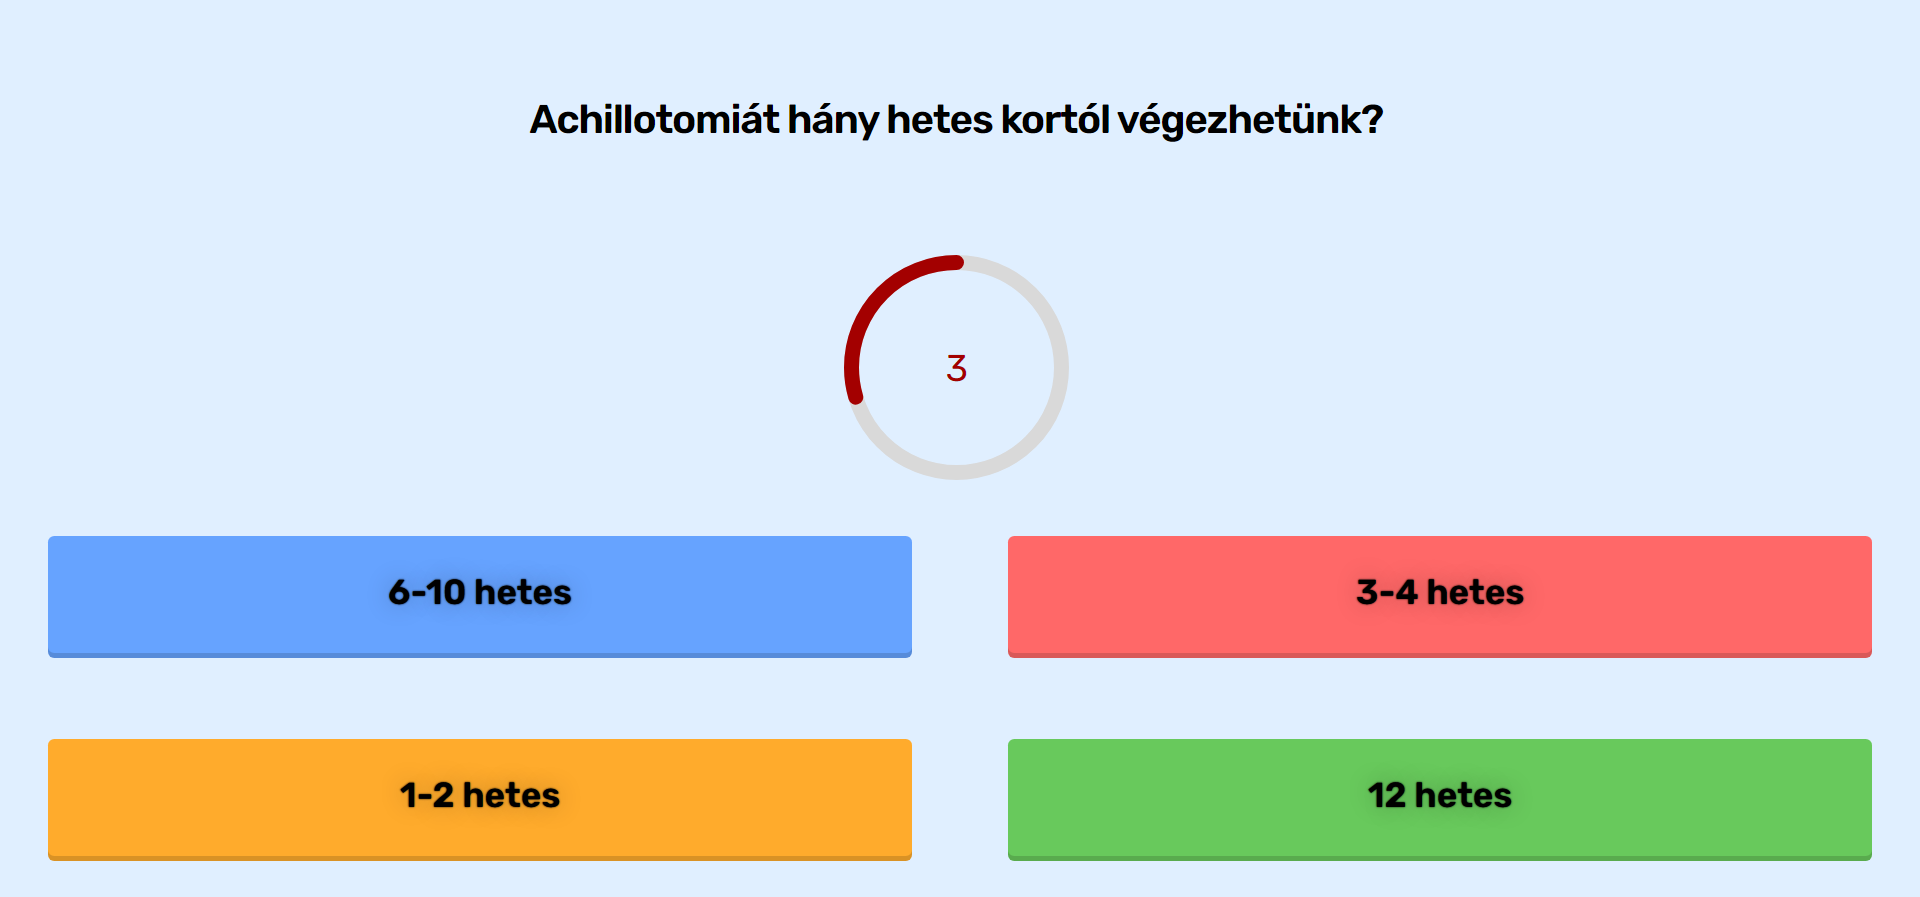
\includegraphics[width=\linewidth]{images/question1.png}
    \caption{Kvíz kérdés}
    \label{fig:question1}
\end{figure}

Majd ezután bejön a kérdés újra viszont a négy válasszal együtt (\prettyref{fig:question1}. ábra). Itt is megy a visszaszámláló. Minden kérdésnél annyi másodperctől kezdődik a visszaszámlálás, amennyit a tesztkészítő definiált a konkrét kérdésre.

\begin{figure}[H]
    \centering
    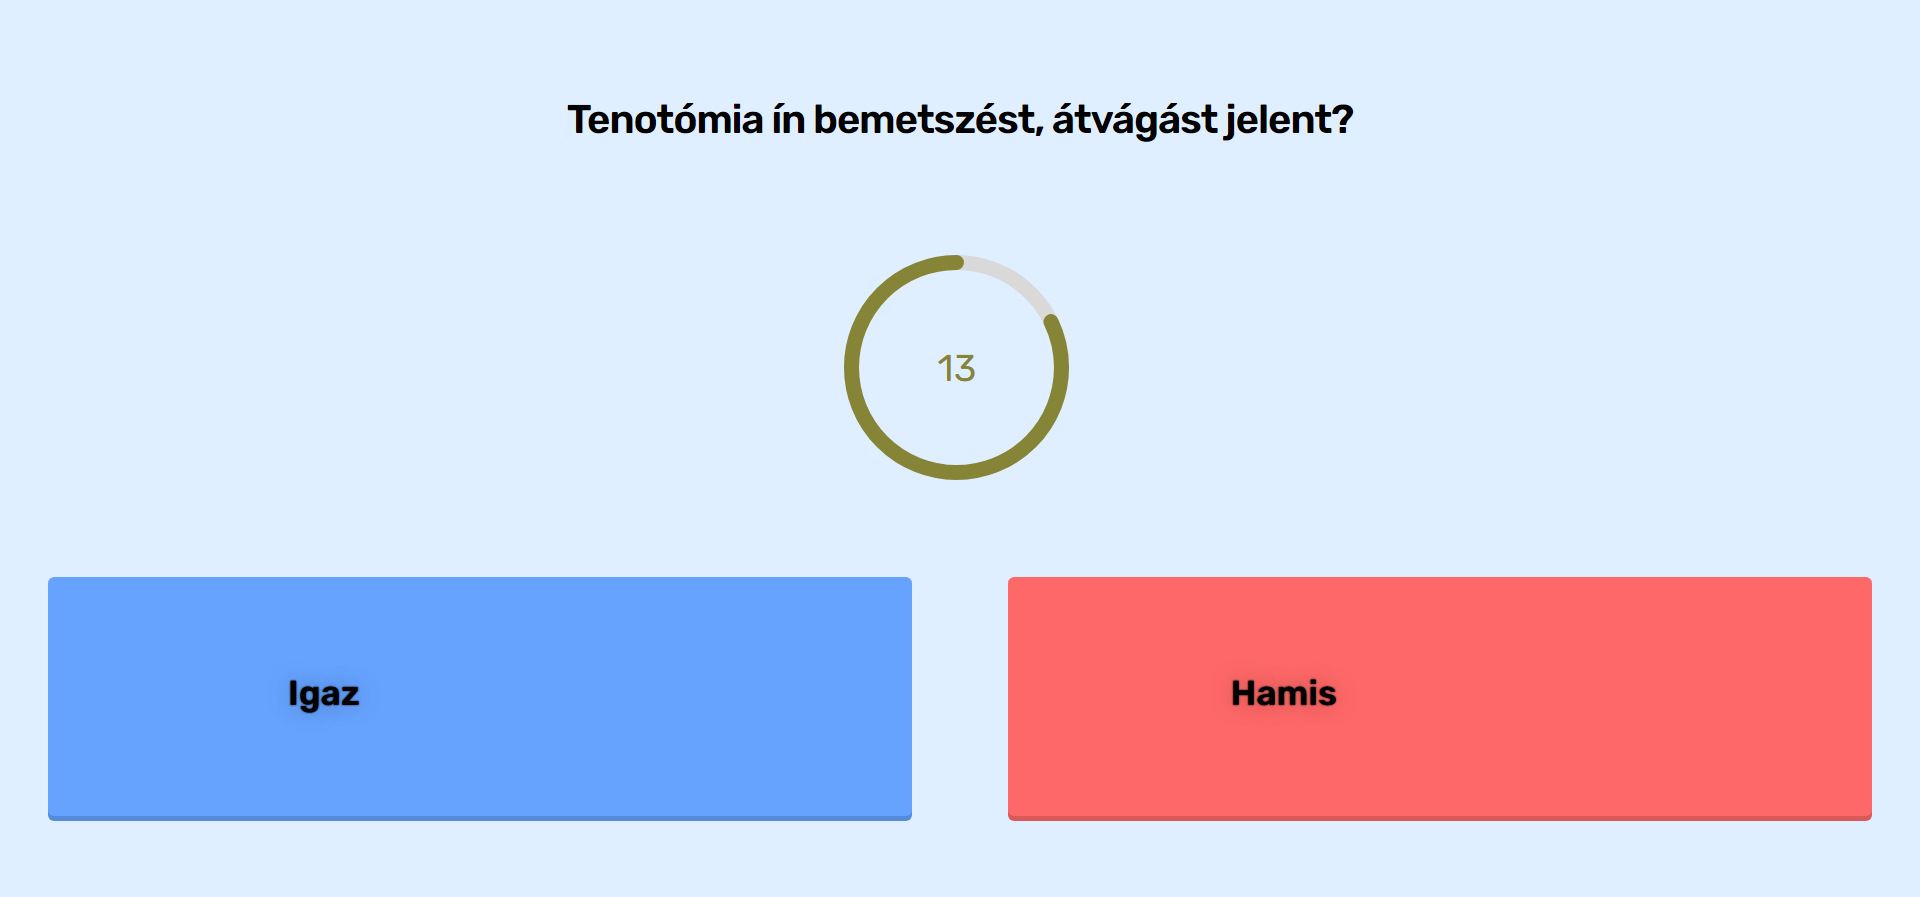
\includegraphics[width=\linewidth]{images/question2.png}
    \caption{Igaz-hamis kérdés}
    \label{fig:question2}
\end{figure}

Egy igaz-hamis kérdés is ugyan így működik, viszont itt csak 2 lehetőség van (\prettyref{fig:question2}. ábra).

\begin{figure}[H]
    \centering
    \begin{subfigure}{0.5\textwidth}
        \centering
        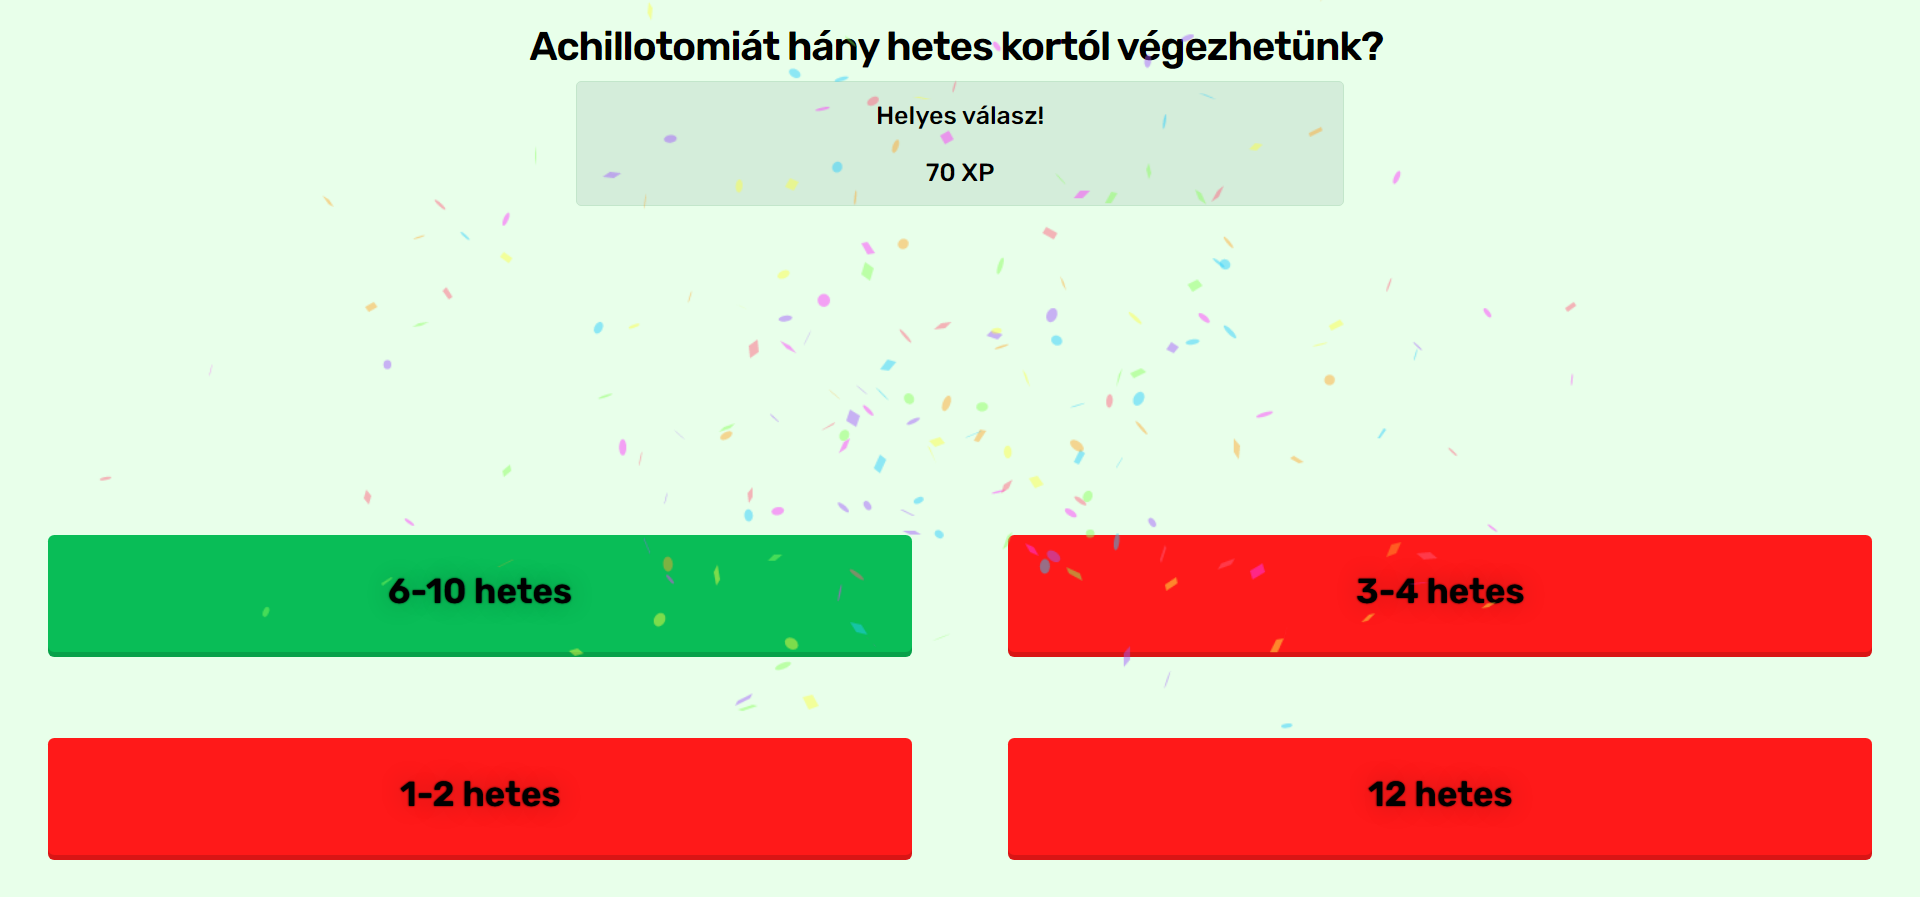
\includegraphics[width=\linewidth]{images/question_good.png}
        \caption{Jó válasz}
    \end{subfigure}%
    \begin{subfigure}{0.5\textwidth}
        \centering
        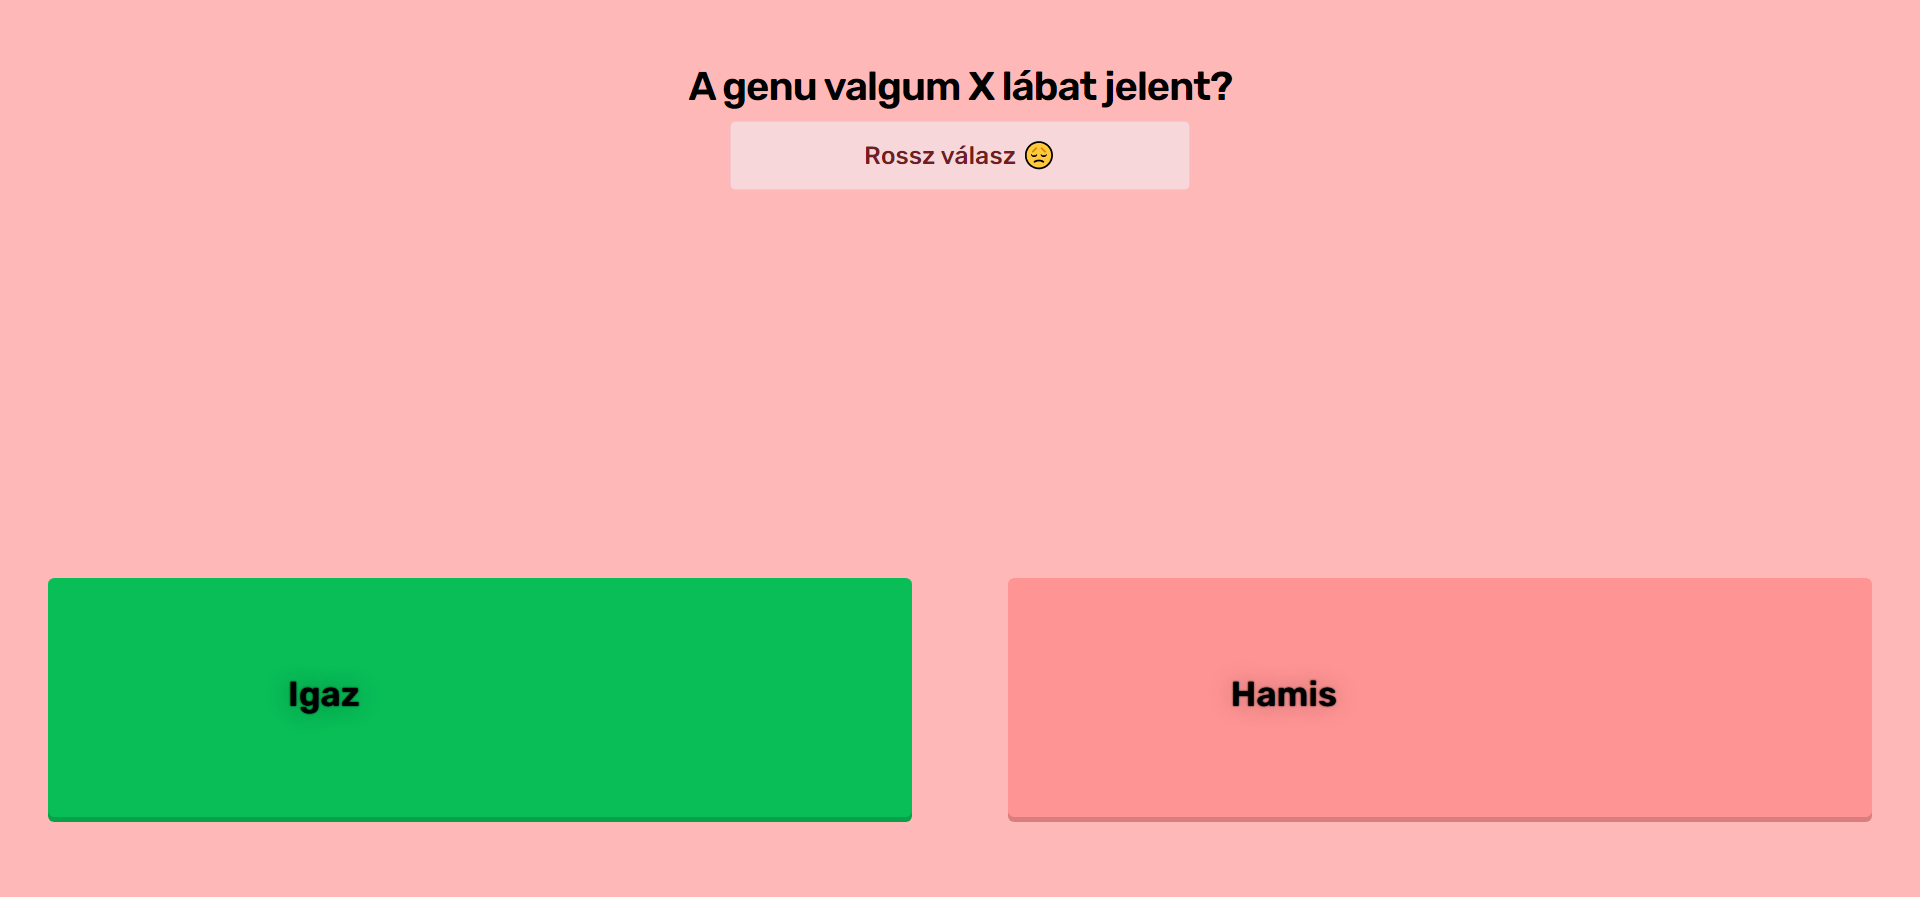
\includegraphics[width=\linewidth]{images/question_wrong.png}
        \caption{Rossz válasz}
    \end{subfigure}
    \caption{Válaszadás}
    \label{fig:question_good_wrong}
\end{figure}

Egy kérdés 3 féleképpen fejeződhet be.
\begin{itemize}
	\item Az első az, ahogy a kép is mutatja \prettyref{fig:question_good_wrong}, hogy jó választ kapunk a kérdésre és megkapjuk a kiérdemelt pontot.
	\item A második, hogy rosszul válaszolunk és nem kapunk semmit.
	\item Az utolsó pedig, hogy nem válaszolunk. Ilyenkor az idő lejárta után, autómatikusan rossz válasznak veszi a rendszer és tovább lép a következő kérdésre.
\end{itemize}

Az XP értéke a helyesség és a sebesség alapján számítható ki.
Jó válasz esetén a pontszámítás az alábbi képlet szerint működik:
\[
\left\lfloor
\dfrac{1}{2} \cdot
\frac
{\text{időkorlát} - \text{maradék idő}}
{\text{időkorlát}}
\cdot \text{xp}
\right\rfloor.
\]
Viszont ha azonnali jó választ adunk, akkor a képleten látható számítás nem megy végbe, hanem megkapjuk az összes lehetséges pontot amit a kérdésre lehet.

\begin{figure}[h!]
    \centering
    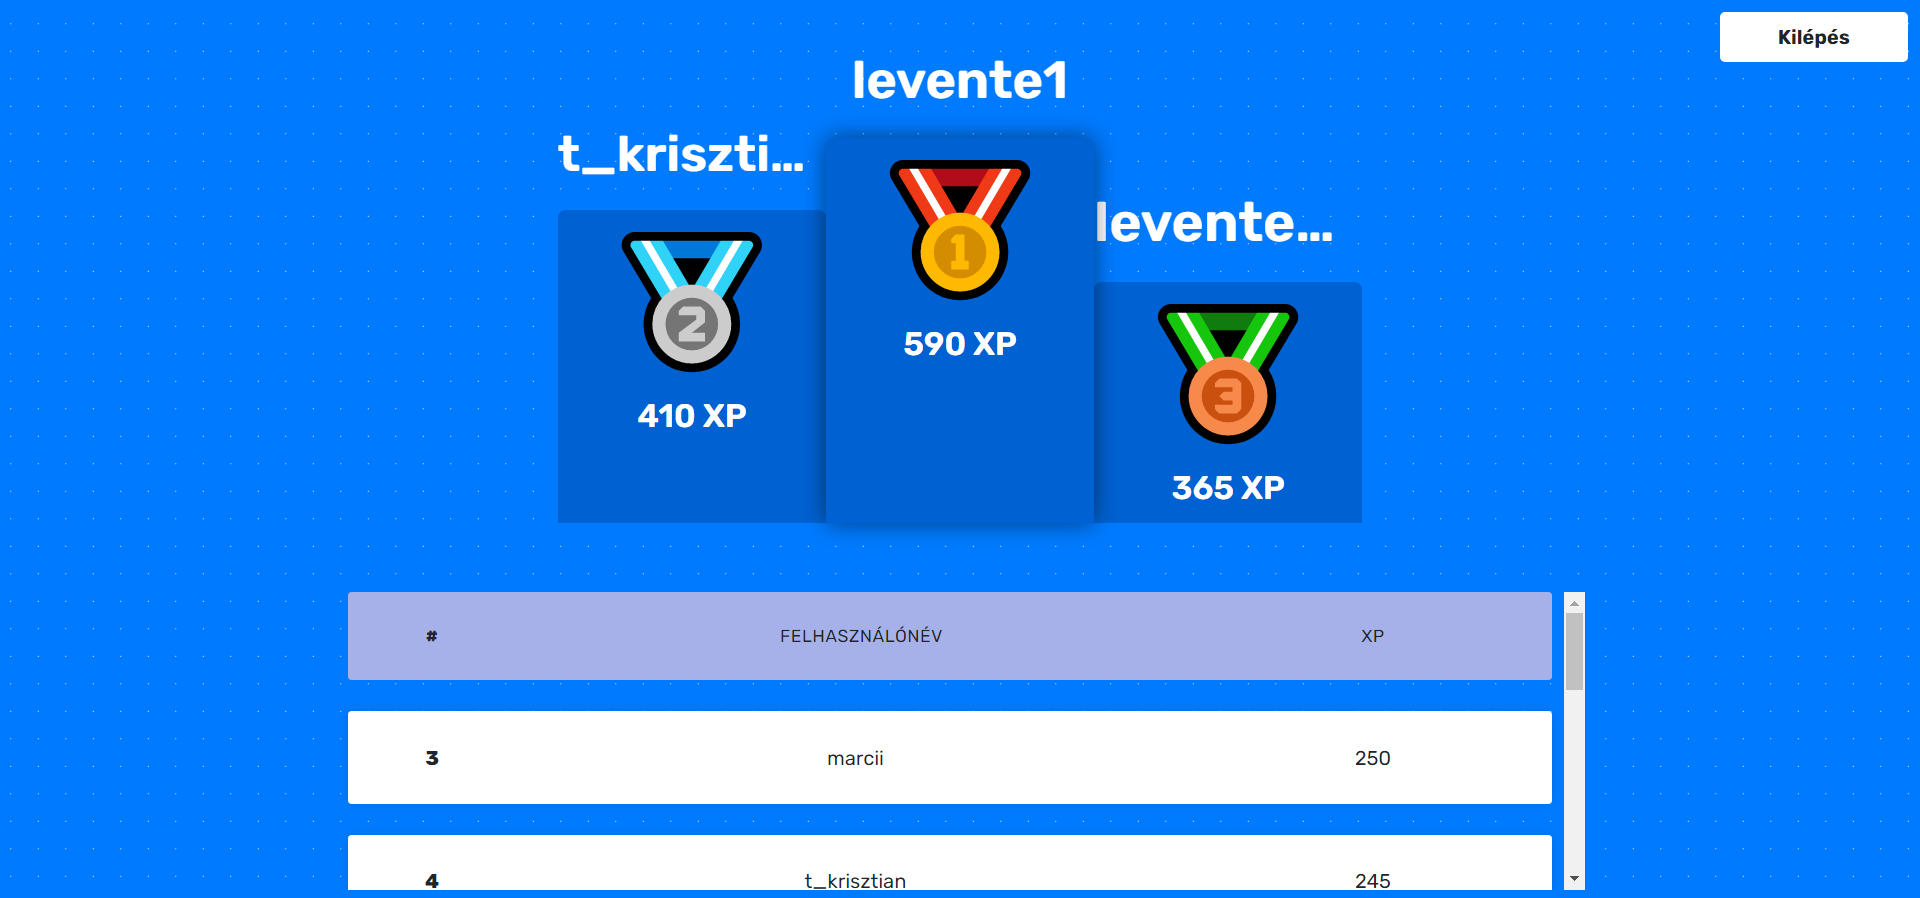
\includegraphics[width=\linewidth]{images/results.png}
    \caption{Eredmények a teszt után}
    \label{fig:results}
\end{figure}

Majd ha az összes kérdés elfogyott, összeadjuk a felhasználó összesen elért pontját és megjelenítjük a többiekével együtt (\prettyref{fig:results}. ábra). Így megnézhetjük, hogy hanyadikok lettünk. Ezután a ,,Kilépés'' gombra kattintva vissza kerülünk a tesztjeinkhez és a főoldalon látjuk, hogy az XP száma növekedett, ha értünk el pontot a teszt kitöltése során.

\Chapter{A backend megvalósítása}

A fejezet részletezi, hogy milyen előnyei miatt esett a választás a .NET Core használatára, majd részletezi a létrehozott adatmodelleket.

\Section{ASP.NET Core}

Az ASP.NET Core egy nagy teljesítményű, nyílt forráskódú, modern, felhőalapú, internetes alkalmazások felépítéséhez használt keretrendszer. Azért jó ez a keretrendszer mert így készen kapjuk az eszközöket a HTTP-szolgáltatások kiépítéséhez, amelyek bármely kliensről elérhetőek, beleértve a böngészőket és a mobileszközöket is. Egy ideális környeztetett biztosít a RESTful alkalmazások felépítéséhez a .NET Framework-el. \newline

Az ASP.NET Core számos fejlesztést kínál az ASP.NET MVC/Web API-hoz képest. Azért választottam, mert a core egy olyan platformokon átívelő webes keretrendszer, amely Windows, macOS, Linux-ra is telepíthető. Így egy elég rugalmas keretrendszer webes és mobilalkalmazásokat vezérlő webes API-k fejlesztésére. Azért is döntöttem az ASP.NET Core mellett, mert biztosítja a megfelelő architektúrát, amihez alkalmazkodva elég gyorsan lehet API-t kreálni. A project létrehozásakor kiválasztottam a Web API projekt sablont, és így már csak annyi dolgom volt, hogy létrehozzam a modelleket amikre szükségem van, és megírjak a hozzájuk tartozó vezérlőket.

\Section{Adatmodellek leképzése}

Az adatbázisban a táblák létrehozásához ,,Code First'' megközelítést alkalmaztam. A helyett, hogy először megterveznénk az adatbázist, majd létrehoznánk azokat az osztályokat amelyek megfelelnek az adatbázis tervezésének. A Code-First megközelítésben az alkalmazás kód részére összpontosít, és ilyenkor osztályokat hozunk létre amelyekből leképződik az adatbázis. Ahhoz, hogy ez létrejöhessen kell egy úgynevezett ORM (\textit{Object-Relational Mapping}) eszköz. A választásom az \textit{Entity Framework}-re esett, mivel ez az egyik legelterjedtebb keretrendszer erre a feladatra. Az Entity Framework az jelen esetben, amely lehetővé teszi, hogy egy adatbázis tábláit C\# osztályokká képezzünk le. \newline

Az API kódjában 6 osztályt hoztam létre amelyekből létre fognak jönni a táblák. Ezek adattagjait részleteztem az \nameref{Adatmodell}. szakaszban.
Viszont a közöttük lévő kapcsolat látszik az említett fejezetben lévő ábrán, de a megvalósításáról kód szinten még nem esett szó. \newline

A \texttt{UsersTest} táblával kezdeném, hiszen ez a fő tábla amely a többit összeköti.
A \texttt{UsersTest}-ben két idegen kulcs van, az egyik a UserId, másik pedig a \texttt{TestId}. Ezekkel kapcsolódik a két legfontosabb tábla, a felhasználó és a teszt. Így a UsersTest segítségével tudjuk azt létrehozni, hogy az, aki az oldalt használja és hozzáadtak egy tesztet, az kap egy példányt a tesztből, így el tudjuk menteni az eredményeit egyesével a meghívottaknak.
Tehát egy \texttt{UsersTest}-hez egy felhasználó és egy teszt tartozik, viszont felhasználókhoz és tesztekhez is több ilyen UsersTest tábla tartozik mivel több ember használja az oldalt és több teszt is van. \newline

A \texttt{User} táblának csak egy idegen kulcsa van ez pedig a RoleId, mivel minden felhasználóhoz tartozik egy jogosultság. \newline

A \texttt{Test}-hez értelemszerűen hivatkozva van maga a kérdés.
\begin{cpp}
[ForeignKey("User")]
public string UserId { get; set; }
public ICollection<Question> Questions { get; set; }
\end{cpp}
Itt egy-több kapcsolat van, melyet úgy valósítottam meg, hogy a \texttt{Test} osztályban létrehoztam egy gyűjteményt, ami egy generikus típus, és ennek a típusparamétere a \texttt{Question} osztály így hivatkozunk rá, hogy itt több kérdés fog tartozni egy teszthez. A másik azonosító pedig a \texttt{UserId}, ami a teszt készítőjének egyedi azonosítóját tartalmazza. \newline

Az \texttt{Answer} táblának pedig két idegen kulcsa van, az egyik a kérdés azonosítója, amiatt, hogy meg tudjuk mondani melyik kérdésre érkezett a válasz. A másik pedig a \texttt{UserTest} azonosítója így vissza tudjuk keresni,  melyik tesztre érkezett a válasz és ki adta a választ, mivel a \texttt{UserTest}-ben benne van a felhasználó azonosítója.

\Section{Az API megvalósítása}

Azt, hogy milyen \textit{endpoint}-okat szeretnék létrehozni, és mi a szerepük, az \nameref{API} szakaszban kifejtettem. Viszont így megvalósítás után be szeretném mutatni néhány elemét az adatküldésnek, hogy lássuk, hogy milyen formában kerülnek a kontrollerhez és miket adunk vissza. 

\SubSection{Felhasználók}

\begin{itemize}[label={$\bullet$}, topsep=0pt, itemsep=0pt, leftmargin=15pt]
    \item[] {\nolinkurl{api/users:}}
          \begin{addmargin}[\parindent]{0pt}
              Bejelentkezéskor a felhasználó email címét és jelszavát elküldve kikeressük, hogy valóban létező, mentett email címet és jelszót küldött el és visszaküldjük a felhasználó adatait. 
              \begin{json}
{
    "email": "teszt@teszt.hu",
    "password": "jelszo000"
}
              \end{json}
              Ha nincs visszaigazolva az e-mail cím \nolinkurl{403}-as, ha rossz adatokat írunk be \nolinkurl{500}-as és ha minden jó akkor \nolinkurl{201}-es kódot kapunk vissza. \newline

              A regisztrációkor elküldött adatok az alábbiak:

              \begin{json}
{
    "roleId": 0,
    "userName": "Levente1999",
    "firstName": "Makszimus",
    "lastName": "Levente",
    "email": "teszt@teszt.hu",
    "password": "Jelszo_.000"
}
              \end{json}

              Miután elküldődnek a felhasználó adatai és vissza lett igazolva az email cím, ami egy link megnyitással jár csak, be is jelentkezhetünk. Ez a link az \nolinkurl{/api/confirm-email} endpoint-ot hívja meg. \newline

              Valamint lehet egy felhasználó adatait módosítani, \nolinkurl{PUT} és törölni, \nolinkurl{DELETE} hívással ugyan azon az endpoint-on: \nolinkurl{/api/users/{userId}}.
          \end{addmargin}
\end{itemize}

\SubSection{Teszt}

\begin{itemize}[label={$\bullet$}, topsep=0pt, itemsep=0pt, leftmargin=15pt]
    \item[] {\nolinkurl{api/tests:}}
          \begin{addmargin}[\parindent]{0pt}
              
              Egy elkészített teszt így néz ki ha elküldjük \nolinkurl{POST}-tal:
              \begin{json}
{
    "title":"Mesterséges intelligencia alapok 2 teszt",
    "description":"Mesterséges intelligencia alapok második zárthelyi dolgozat",
    "userId":"165",
    "created":"2021-01-12",
    "deadline":"2021-01-22",
    "questions":[
        {
            "problem":"A Turing-teszt teljesítéséért járó arany medál a díj kitűzőjét, Hugh Loebnert ábrázolja?",
            "answerOne":"true",
            "answerTwo":"false",
            "timeLimit":5,
            "xp":3,
            "correctAnswer":0
        }
    ]
}
              \end{json}
          \end{addmargin}
\end{itemize}

\newpage

\SubSection{Kérdések}

\begin{itemize}[label={$\bullet$}, topsep=0pt, itemsep=0pt, leftmargin=15pt]
    \item[] {\nolinkurl{api/questions:}}
          \begin{addmargin}[\parindent]{0pt}
              A teszt készítésekor minden kérdést egyesével küldünk el ide, a következő adattagokkal:
              \begin{json}
{
    "problem": "Ha csinálnánk egy csoportos IQ tesztet egy tankör hallgatóival mennyi lenne az átlag?",
    "answerOne": "110",
    "answerTwo": "120",
    "answerThree": "130",
    "answerFour": "140",
    "timeLimit": 10,
    "xp": 5,
    "correctAnswer": 0
}
              \end{json}
          \end{addmargin}
\end{itemize}

\SubSection{Válaszok}

\begin{itemize}[label={$\bullet$}, topsep=0pt, itemsep=0pt, leftmargin=15pt]
    \item[] {\nolinkurl{api/answers:}}
          \begin{addmargin}[\parindent]{0pt}
              Itt egy teszt kérdés válaszának küldésekor csak egy egyszerű, négy számot tartalmazó objektum, ahol a kérdés és a felhasználói teszt azonosítója adja az egyediségét minden válasznak. Emellet elküldjük még azt, hogy milyen gyorsan válaszolt, és hogy mi volt a válasza.

              \begin{json}
{
    "questionId": 1,
    "usersTestId": 2,
    "responseTime": 5,
    "userAnswer": 4
}
              \end{json}
          \end{addmargin}
\end{itemize}

\SubSection{Felhasználó tesztjei}

\begin{itemize}[label={$\bullet$}, topsep=0pt, itemsep=0pt, leftmargin=15pt]
    \item[] {\nolinkurl{api/users-tests:}}
          \begin{addmargin}[\parindent]{0pt}
            Egy felhasználói teszt lekérés a felhasználó id-jának elküldésével történne és ezt kell visszakapnunk:
              \begin{json}
{
    "id": 1,
    "userId": 1,
    "testId": 1,
    "test": {
        "id": 1,
        "description": "A tesztben csak kvíz kérdések szerepelnek, tehát 4 választási lehetőség közül kell majd választaniuk. Eredményes munkát kívánok!",
        "userId": "152",
        "title": "Mesterséges intelligencia alapok 2 teszt",
        "created": "2021-01-12T00:00:00",
        "deadline": "2021-01-22T00:00:00",
        "questions": [
            {
                "id": 1,
                "problem": "Ha csinálnánk egy csoportos IQ tesztet egy tankör hallgatóival mennyi lenne az átlag?",
                "answerOne": "110",
                "answerTwo": "120",
                "answerThree": "130",
                "answerFour": "140",
                "timeLimit": 10,
                "xp": 5,
                "correctAnswer": 0
            },
            {
                "id": 2,
                "problem": "A Turing-teszt teljesítéséért járó arany medál a díj kitűzőjét, Hugh Loebnert ábrázolja?",
                "answerOne": "true",
                "answerTwo": "false",
                "answerThree": null,
                "answerFour": null,
                "timeLimit": 5,
                "xp": 3,
                "correctAnswer": 0
            }
        ]
    },
    "finished": "2021-01-13T00:00:00",
    "earnedXp": 6
}
              \end{json}

              Amikor egy felhasználó befejezi a tesztkitöltést, akkor itt módosításra kerül az XP adattag és megjelenik egy rangsor, hogy ki hány pontot ért el. Ehhez le kell kérni az összes játékost akik kitöltötték a tesztet. Ezt megtehetjük a \nolinkurl{api/users-tests/test/testId} \textit{endpoint}-on. A főoldalon szereplő kitöltött és kitöltetlen tesztek számát is innen tudjuk lekérni.
          \end{addmargin}
\end{itemize}

\Section{Session tárolása}

A régi ASP.NET-től eltérően az ASP.NET Core nem rendelkezik \lstinline{Cache} objektummal. Az ASP.NET Core azonban számos különféle gyorsítótár-támogatást nyújt. Ilyen lehet a memóriában, az elosztott gyorsítótárban vagy a válasz-gyorsítótárban tárolt. \newline

Az elosztott SQL Server-es gyorsítótár megvalósítása lehetővé teszi az elosztott gyorsítótár számára, hogy az SQL Server adatbázist használja háttértárként. Először ezt hozzá kell adni a \lstinline{Startup.cs} file-hoz:

\begin{cpp}
    services.AddDistributedSqlServerCache(options => {
        options.ConnectionString =
            Configuration.GetConnectionString("TestMEApiContext");
        options.SchemaName = "dbo";
        options.TableName = "Session";
    });
\end{cpp}

SQL Server gyorsítótárazott cache létrehozásához egy SQL Server példányban használni kell az \lstinline{sql-cache} eszközt. Először létre kell hozni egy táblázatot az SQL Server kiszolgálón az \lstinline{sql-cache create} parancs futtatásával. Meg kell adni az SQL Server példányt, az adatbázist, a sémát (például dbo) és a tábla nevét (például Session) \cite{distributedSQLServerCache}:

\begin{cpp}
    dotnet sql-cache create "Data Source=(localdb)\MSSQLLocalDB;Initial
    Catalog=DistCache;Integrated Security=True;" dbo Session
\end{cpp}

Így hoztam létre a táblát amiben az összes bejelentkezett felhasználó session-je tárolódik.
